\chapter{Framework EPUBKit}
\section{Tworzenie frameworku na iOS}

Tworzenie bilioteki którą zamierzamy następnie wykorzystać we własnej aplikacji lub udostępnić publiczne, jest stosunkowo prostym procesem. Wszystko sprowadza się do stworzenia nowego projektu w Xcode a następnie dołączenie go do przestrzeni roboczej (Xcode Workspace) w której znajdzie się projekt aplikacji nad którą pracujemy oraz projekt biblioteki. Aby stworzyć projekt biblopteki należy uruchomić Xcode IDE i na powitalnym ekranie wybrać opcję "Create a new Xcode project" która przeniesie nas do kolejnego ekranu z możliwością wybrania konktetnego szablonu projektu nad jakim chcemy pracować.

\begin{figure}[ht!]
  \centering
  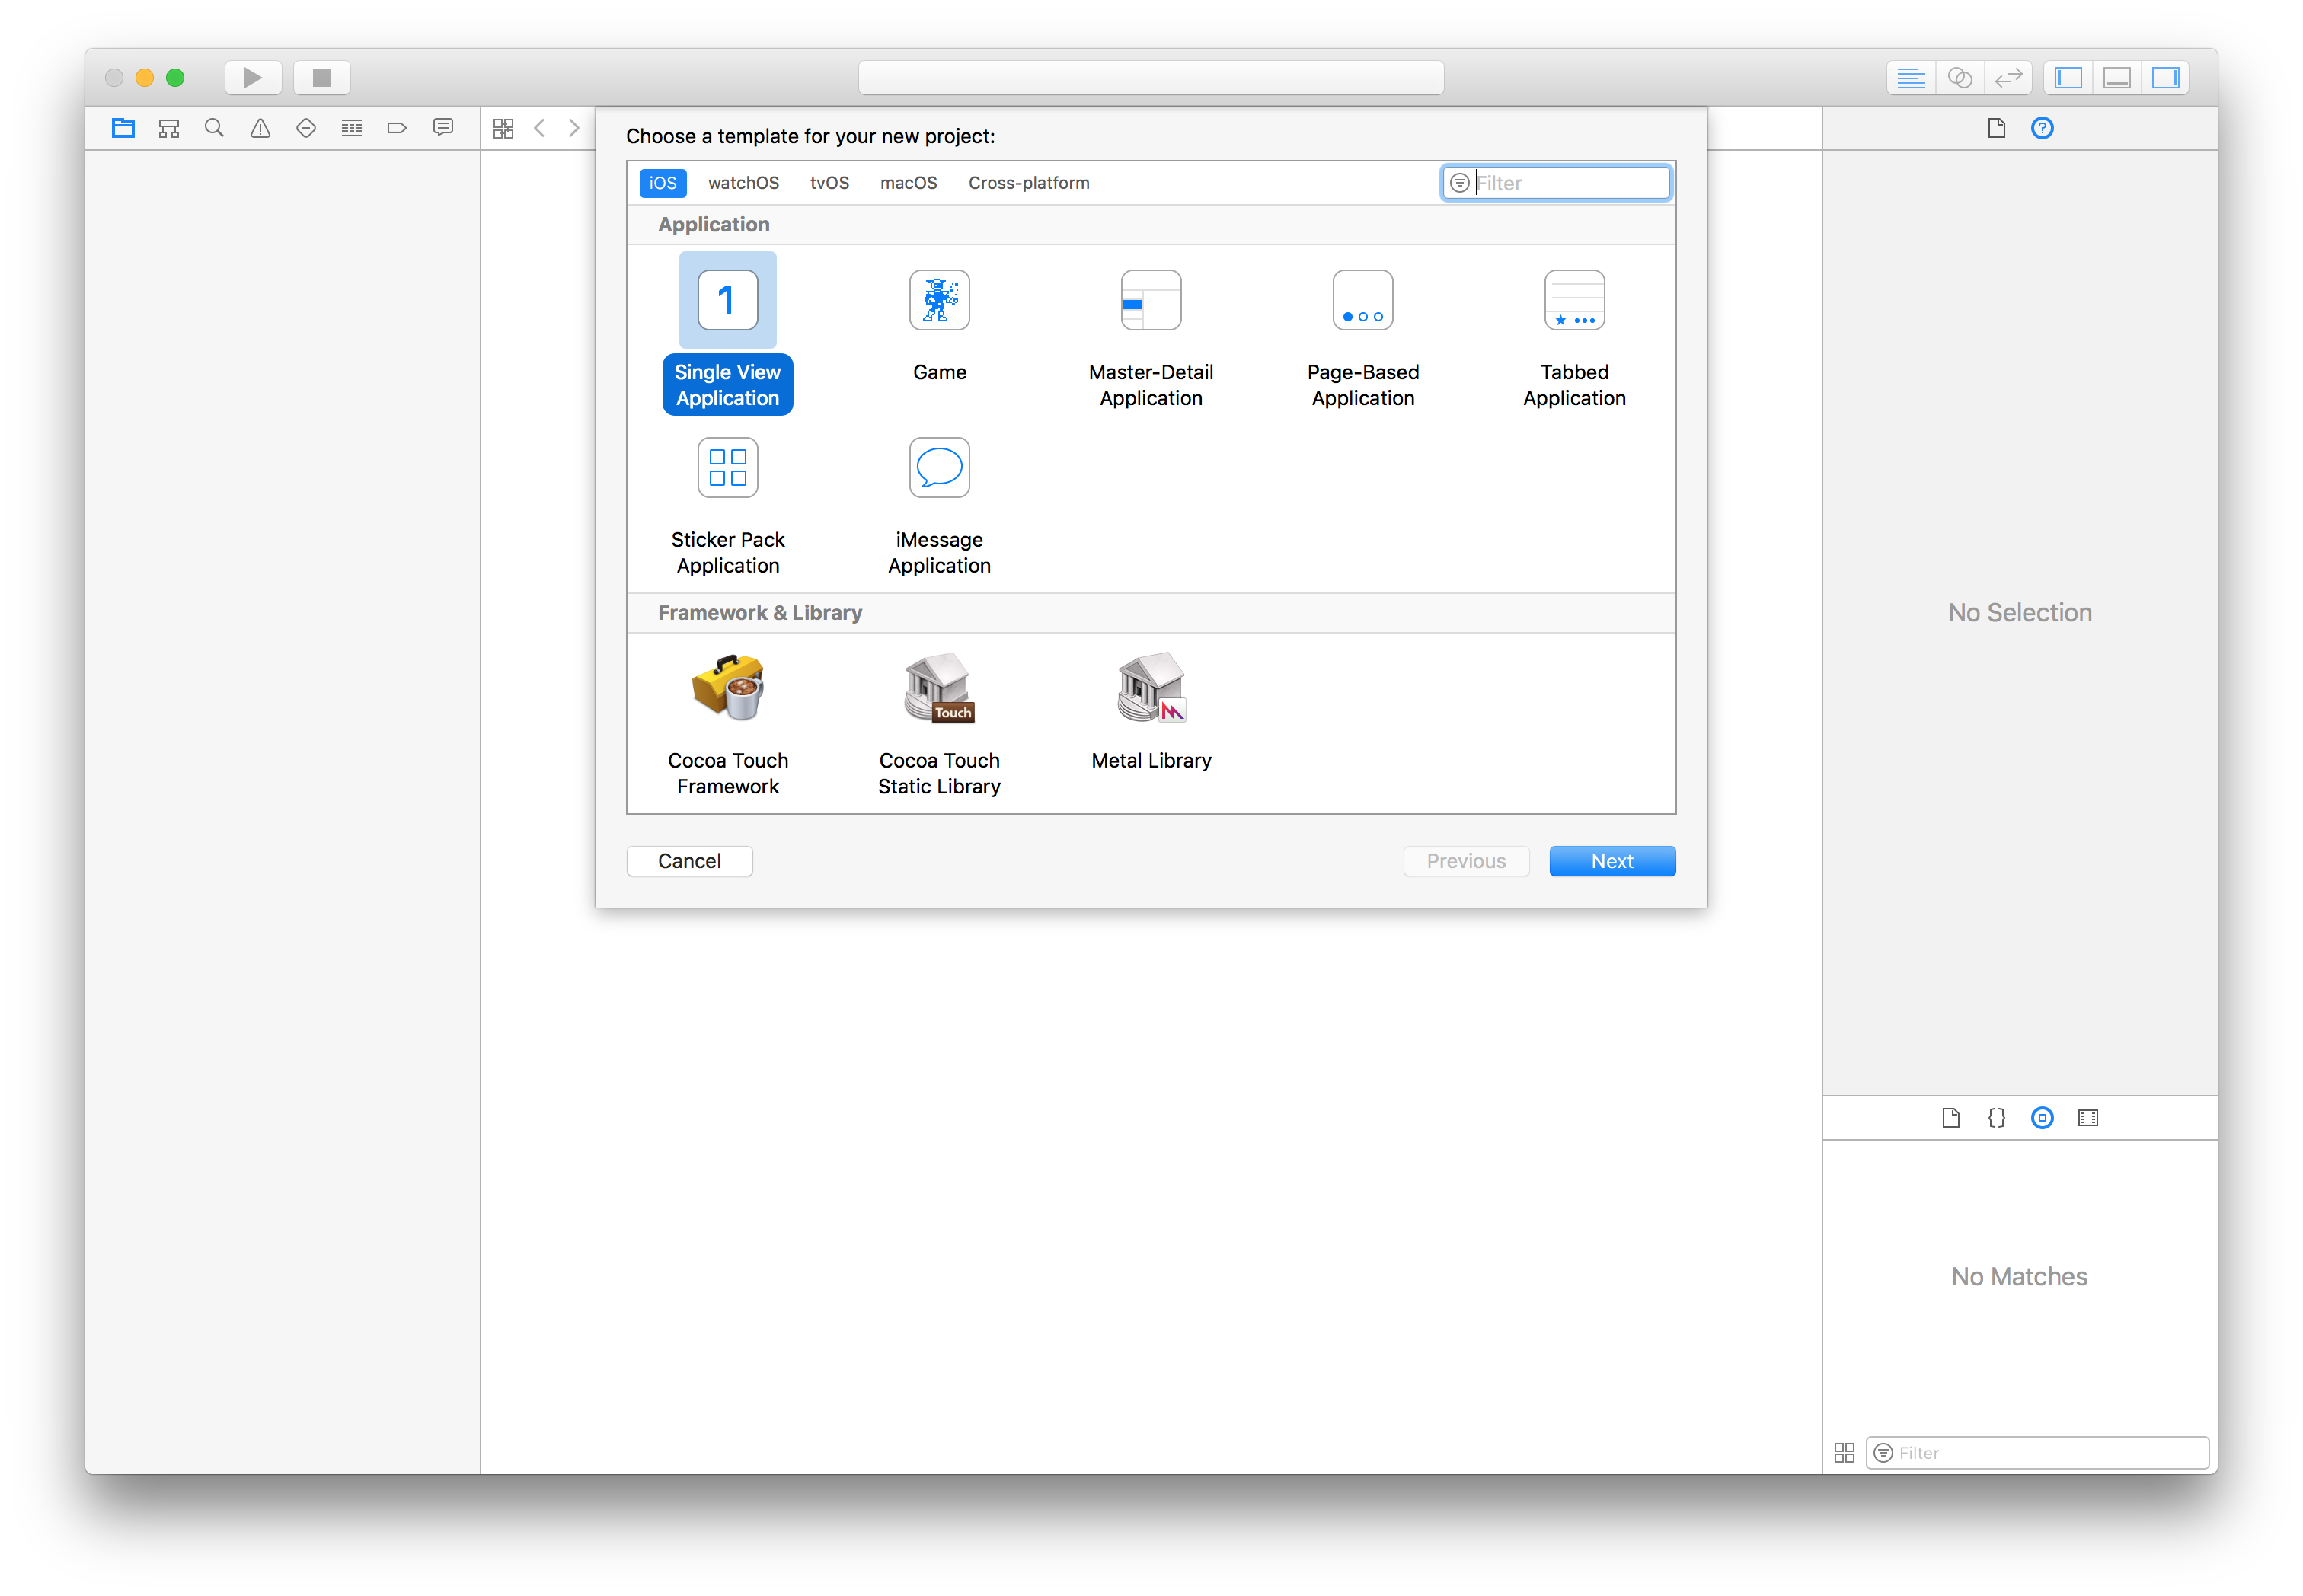
\includegraphics[width=120mm]{images/chapter-4-image-1-new-project.png}
  \caption{Szablny projektów które znajdują się w Xcode}
  \label{chapter-4-image-1-new-project}
\end{figure}

Na naszym przypadku interesuje nas szablon "Cocoa Touch Framework", a po jego wybraniu jesteśmy proszeni o uzupełnienie formularza ze szczegółowymi informacjami na temat projektu który zamierzamy stworzyć, poczynając od nazwy, po język w którym będzie napisany (Swift lub Objective-C). Następnie Xcode poprosi o wskazanie lokalizacji na dysku w której chcemy zapisać projekt oraz zapyta nas czy chcemy stworzy repozytorium systemu kontroli wersji git. W tym momencie mamy projekt który można już w prosty sposób dołączyć do aplikacji (Co zostanie opisane w kolejnym rozdziale przy okazji omawianie wykorzystania biblioteki EPUBKit w demonstracyjnej aplikacji). Teraz już możemy tworzyć klasy które mają składać sie na funkcjonalność biblioteki.

\begin{figure}[ht!]
  \centering
  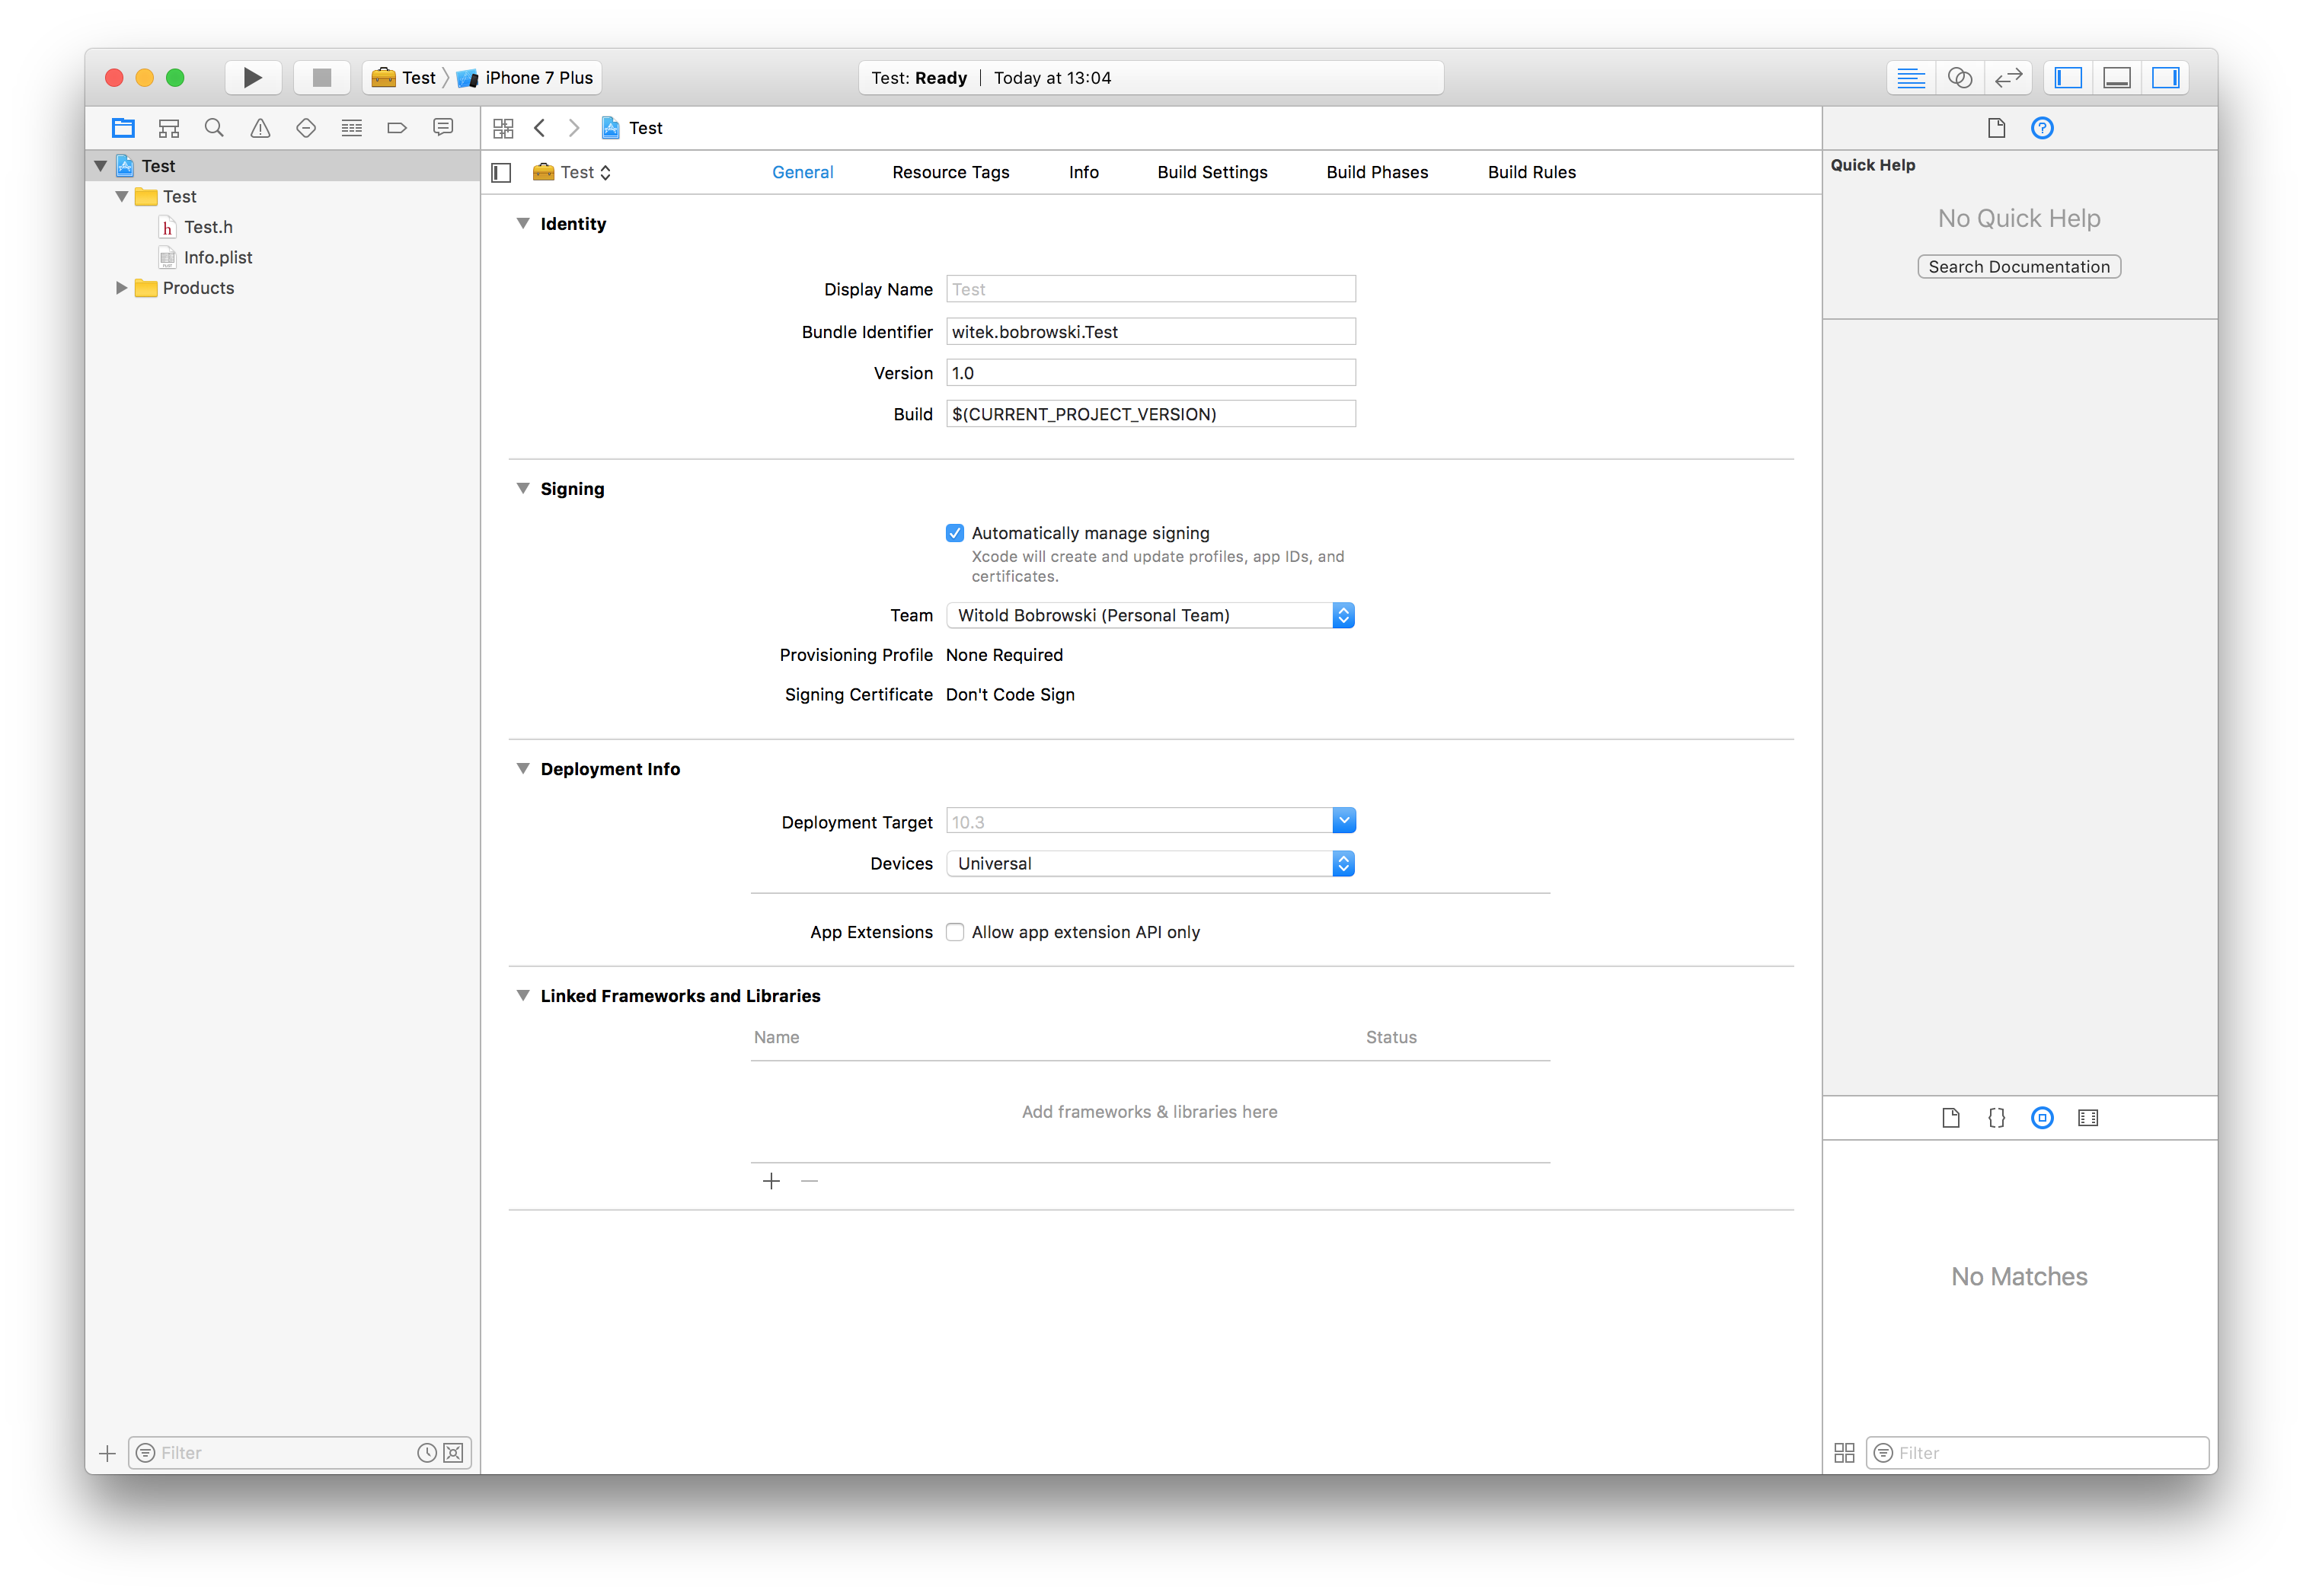
\includegraphics[width=120mm]{images/chapter-4-image-2-empty-project.png}
  \caption{Szablny projektów które znajdują się w Xcode}
  \label{chapter-4-image-1-new-project}
\end{figure}

Plik projektu pozwala nam za szczegółowy wgląd w preferencje oraz infromacje jego dotyczące, które można zmieniac w dowolnej chwili. Jest możliwość zmiany wersji bibioteki, docelowego urządzenia (iPhone lub iPad), preferowanej wersji systemu który ma wspierać bibltioteka, oraz co bardzo istotne, mamy możliwość użycia innych niezależnych bibliotek w naszym projekcie. Wystarczy wyeksportować plik projektu jako plik przestrzebi roboczej do której można dodać inne projekty a następnie połączyć je z naszym w menu "General" w polu "Linked Frameworks and Libraries" w pliku projektu. Dzięki tak funkcjonalnym i prostym w obsłudze narzędziom jak Xcode, po szybkiej konfiguracji swoją uwagę można skupić na samej logice którą chcemy zaimplementować.

W tym rozdziale zostanie opisana stworzna przez mnie biblioteka EPUBKit. Biblioteka ta jest oparta na architekturze MVC (Model View Controller) dlatego omówienie jest rozpocznę od opisania jej modelu oraz parsera, a następnie przejdę do zawartych w niej widokach które pozwalają na wyświetlenie danych zawartych w modelu. Zakończę rozdział przedstawiając możliwości dystrybuowania takiej biblioteki, przy pomocy szeroko stosowanych i popularnych narzędzi, które są podstawą iOS developmentu.

\section{Model}

Struktura klas modelu została zaprojektowana w ten sposób aby z jednej strony odzwierciedlała struktrę dokumnetu EPUB oraz format OPF który EPUB wykorzystuje, a z drugiej by trzymała się konwencji swiftowych i intuicyjnie reprezontowała obiekt który następnie będzie wykorzystywany w kolejnych klasach biblioteki.

\begin{lstlisting}[caption={Struktura modelu EPUBKit.}, language=bash]
    Model
    |-- EPUBDocument.swift
    |-- EPUBManifest.swift
    |-- EPUBMetadata.swift
    |-- EPUBSpine.swift
    `-- EPUBTableOfContents.swift
\end{lstlisting}

\subsection{EPUBDocument}
\subsection{EPUBManifest}
\subsection{EPUBMetadata}
\subsection{EPUBSpine}
\subsection{EPUBTableOfContents}


\section{Parser}

\section{Widok}

\section{Dystrybucja}
